\section{The Problem}

\par
As early as 1783, invisible structures in the Universe has been hypothesised, but it wasn't until the end of the 19th century, when astronomical photography was realised that observations gave a hint of an invisible mass  \cite{History_Of_Dark_Matter_2018_ref}.
These hints at an unknown have grown over the previous century from a minor puzzle that could perhaps be explained away by observational uncertainties to a challenge to fundamental particle physics, cosmology and astrophysics.
Here some of the evidence is explored.

%Some other quotes like
%\par
%Perhaps the most fitting conclusion to this was by Lord Kelvin who concluded
%
%\begin{quote}
%    many of our stars, perhaps a great majority of them, may be dark bodies
%\end{quote}
%
% Add Quote about black holes 17XX :P 


\subsection{Galactic Scale}

\par
Some of the earliest indications of dark matter comes from comparing methods used to estimate the mass of astronomical bodies.
Once such example of this comes from Zwicky, who in 1933 who sought to determine the mass of the Coma Cluster by relating the potential energy to the kinetic energy using the virial theorem.
Zwicky found that in order to achieve the average observed velocity of 1000 km/s, there would need to be in excess of ~ 12 times more mass than estimated using the galaxy radius and 400 times the mass estimated from luminous matter \cite{Fritz_Zwicky_1933_ref}.
This lead to the conclusion that; 
\begin{quote}
"If this should be verified, it would lead to the surprising result that dark matter
exists in much greater density than luminous matter."
\end{quote}
which, although not the first time the phrase "dark matter" had been used is perhaps the most well known instance.
Modern techniques have found issues with the calculations used by Zwicky but the most significant finding of the missing mass has not been dis-proven.

\par
Shortly after, in 1941, it was shown that galactic rotation curves could be used as a reliable way of determining the mass distribution within a galaxy \cite{Chandrasekhar_1941_ref}.
From standard Newtonian dynamics, an object in circular motion with mass $m$ has rotation velocity $v$ that follows;
\begin{equation}
    v(r) = \sqrt{\frac{rF}{m}} = \sqrt{\frac{GM(r)}{r}}
    \label{eq:Kepler_Motion}
\end{equation}
where $G$ is the gravitational constant and $M(r)$ is the mass contained within the radius $r$ given by; $M(r) = 4 \pi \int \rho(r) r^{2} dr$.
In a spiral galaxy, the luminous mass is distributed as approximately a disc. 
Using this, we expect the tangential velocity of an object within the galaxy to increase with the radius until the there is equal mass pulling in and out.
After this point the velocity of the object should decrease as $\sqrt{\frac{1}{r}}$ as it becomes further away from the majority of the mass.
However, observations have shown that this is in fact not the case, and instead the velocity distribution remains flat as illustrated in Figure \ref{fig:DM_Evidence_NGC_6503}.
\begin{figure}[!htbp]%
    \centering
    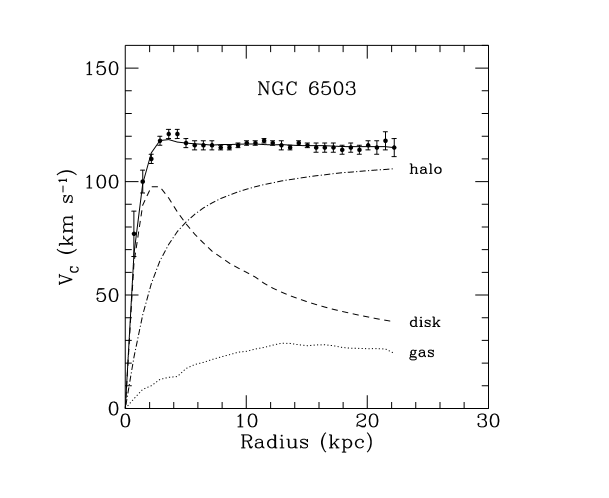
\includegraphics[scale=1.0]{Figures/DarkMatterEvidence/NGC_6503_galaxy_speed.png}
    \caption{Galaxy rotation curve for the NGC 6503 galaxy along with different mass distribution models which together produce the fit on the observed data. The measurements are from 1991. Figure adapted from \cite{NGC_6503_galaxy_rotation_ref}}
    \label{fig:DM_Evidence_NGC_6503}
\end{figure}
These measurements have been performed multiple times and redone with modern measurements, but always producing results inconsistent with the majority of the mass being in the luminous disc.
Instead, what is suggested is that there is an invisible halo which has a mass density following $\rho(r) \alpha \frac{1}{r^2}$ at large $r$.
This is in fact a topic on ongoing research which now focuses on Low Surface Brightness galaxies, where dark matter is the dominating component \cite{MHONGOOSE_2018_ref}.


\subsection{Galaxy Cluster Scale}
\par
At a largest scale, the discrepancy between the luminous mass and the inferred mass becomes even more apparent.
The general theory of relativity tells us that space-time is warped by the presence of mass.
As such, light propagating along null-geodesics will curve when near any object with mass, with the degree of curving being directly correlated to the intervening objects mass.
This effect, known as gravitational lensing, can be categorised as strong, weak or microlening\footnote{Strong lensing typically produces multiple images of the same object. Weak lensing has no noticeable distortion but can be discovered by statistically. Microlensing is when a significantly smaller object produces a distortion.}. 
Gravitational lensing manifests itself in observations as duplicate features and distortions.
An example of strong lensing is shown in Figure \ref{fig:DM_Evidence_Einstein_Ring} where light from a distant galaxy has been distorted into an arc due to the mass of an intervening galaxy.

\begin{figure}[!htbp]%
    \centering
    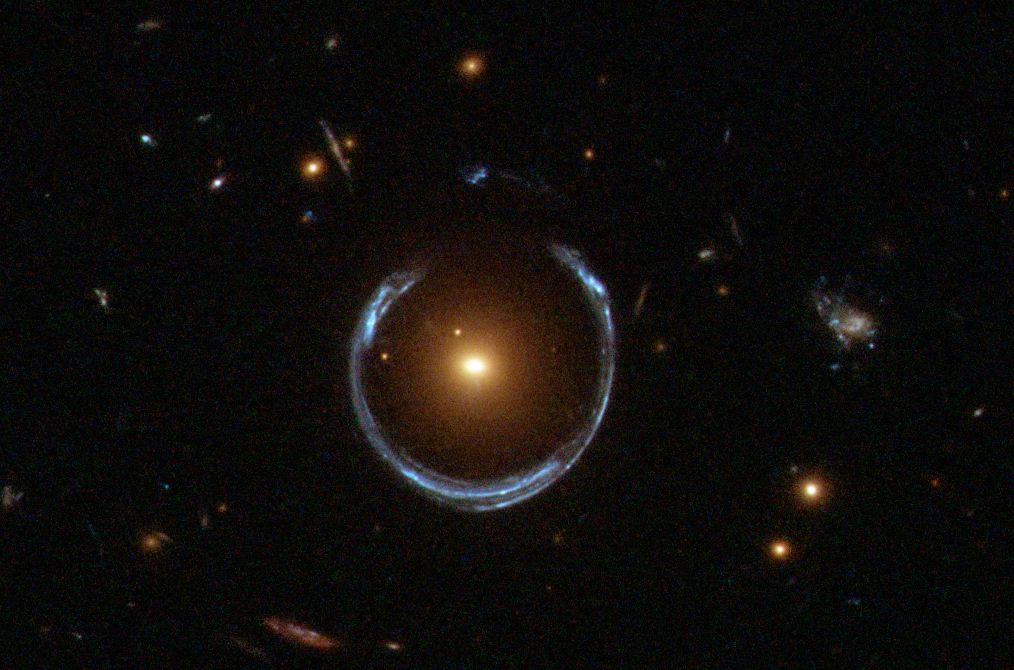
\includegraphics[scale=0.5]{Figures/DarkMatterEvidence/Einstein_Ring_from_Hubble.JPG}
    \caption{An example of a "Horseshoe Einstein Ring" created by the bending of light from a distant blue galaxy by the central red galaxy LRG 3-757. [ESA/Hubble]}
    \label{fig:DM_Evidence_Einstein_Ring}
\end{figure}

Based on the amount of distortion, the mass of the object causing the lensing can be measured and can be applied to both individual galaxies as well as clusters.
The mass required for the lensing observed can then be compared to the luminous mass.
The studies have all found that there is a significant missing mass in cluster and galaxies.

\par
Another example of this is Cluster 1E0657-558, also known as the Bullet Cluster.
This galaxy cluster was formed by the merger of two smaller clusters as shown in Figure \ref{fig:DM_Evidence_Bullet_Cluster}.
In this collision, the baryonic matter can be tracked via electromagnetic radiation and the mass components by lensing.
What is observed is that there is a discrepancy between the two distributions; with the luminous matter appearing to have mixed during the collision causing the matter to slow down.
On the other hand, the majority of the mass has passed through.
What this indicates is that in addition to there being a significant invisible mass, this mass must also have a very small cross-section with baryonic matter and itself.
\begin{figure}[!htbp]%
    \centering
    \caption{Bullet Cluster}
    \label{fig:DM_Evidence_Bullet_Cluster}
\end{figure}


\subsection{Cosmological Scale}
\par
What is often quoted as the strongest evidence for dark matter comes from the cosmic microwave background (CMB) radiation which was first discovered in 1965.
This is a near perfectly uniform field of microwave photons with the energy spectrum of a 2.7225K blackbody.
These photons, sometimes referred to as 'relic' radiation, last interacted with with the early Universe, some 380,000 years after the Big Bang\footnote{The surface of last scattering}, before the Universe cooled sufficiently for recombination\footnote{When electrons were first able to bind to nuclei} and neutral Hydrogen formation.
At this time, the Universe was filled with a plasma as there was enough energy to ionise an atom as soon as it has been formed.
The CMB photons decoupled from the plasma during this time and was able to were able to free-stream through the Universe.
As the Universe has expanded, these photons have red-shifted down to the now observed microwave photons.
Maps of the CMB have been undertaken by multiple satellite missions, of which ones is shown in Figure \ref{fig:DM_Evidence_CMB_Map}.

\begin{figure}[!htbp]%
    \centering
    \caption{Bullet Cluster}
    \label{fig:DM_Evidence_CMB_Map}
\end{figure}

The CMB is very uniform, as the Universe was very isotropic at the moment the CMB decoupled. 
However, there are very small anisotropies at the 0.02\% level.




%\subsection{Nucleosynthesis}
%\par
%Immediately after the Big Bang, the temperature of the primordial plasma was %sufficiently high such that free protons and neutrons were in thermal equilibrium;

%\begin{equation}
%\begin{aligned}
%    n + \nu_{e} \rightleftharpoons p + e^{-} \\
%    n + e^{+} \rightleftharpoons p + \overline{\nu}_{e} \\
%    n \rightleftharpoons p + e^{-} + \overline{\nu}_{e}
%\end{aligned}
%\end{equation}
